\subsection{Problem 4}
\subsubsection{Species and environment prediction model}

On the basis of Problem 3, another expression of Lotka-Volterra model is used as follows:
\begin{equation}\label{4.1}
    \left\{
    \begin{array}{l}
        \frac{dx_{1}(t)}{dt}=x_{1}(t)[r_{10}-a_{11}x_{1}(t)-a_{12}x_{2}(t)] \\
        \frac{dx_{2}(t)}{dt}=x_{2}(t)[r_{20}-a_{21}x_{1}(t)-a_{22}x_{2}(t)]  \\
        x_{i}(t)>0, r_{i0}>0, a_{ij}>0,(i=1,2;j=1,2).
    \end{array}
    \right.
    \end{equation}

Where,

$x_{1}(t)$ and $x_{2}(t)$ are the scale of fungi 1 and 2 at time $t$ (described by number);

$r_{i}(0)$ is the growth rate within the population;

$a_{ij}$ is the competition coefficient within the population (when $i=j$) or the competition coefficient between the populations (when $i\neq j$).

Let $C_{0}(t)$ represent the amount of external factors influencing individuals at time $t$, and $C_{c}(t)$ represent the amount of external factors influencing the environment at time $t$. Assuming that the fungal population does not migrate and is homogeneous and introduces random disturbance, then:
\begin{equation}\label{}
    r_{i0} \to r_{i0} + \sigma_{i}^2 dB_{i}(t)
\end{equation}

Where,

$dB_{i}(t)$ is the interference of external variables;

$\sigma_{i}^2$ is Brown's exercise intensity.

The following stochastic population dynamic system is introduced into Equation (\ref{4.1}):
\begin{equation}\label{4.2}
    \left\{
    \begin{array}{l}
        dx_{1}(t)=x_{1}(t)[r_{10}-r_{11}C_{0}(t)-a_{11}x_{1}(t)]dt-x_{1}(t)a_{12}x_{2}(t)+\sigma_{1}x_{1}(t)dB_{1}(t) \\

        dx_{2}(t)=x_{2}(t)[r_{20}-r_{21}C_{0}(t)-a_{21}x_{1}(t)]dt-x_{2}(t)a_{22}x_{2}(t)+\sigma_{2}x_{2}(t)dB_{2}(t) \\
        x_{i}(t)>0,i=1,2
    \end{array}
    \right.
    \end{equation}

$r_{i1}$ is the influence intensity of external factors on the dynamical system.

Through transformation, we can get:
\begin{equation}\label{4.3}
    \left\{
    \begin{array}{l}
        \frac{dC_{0}(t)}{dt}=kC_{c}(t)-(g+m)C_{0}(t) \\
        \frac{dC_{c}(t)}{dt}=-hC_{c}(t)+u(t) \\
    \end{array}
    \right.
    \end{equation}

The initial values of the two influences are $C_{0}(0)=C_{c}(0)=0$

Where,

$k,g,m,h$ are all normal numbers;

$kC_{c}(t)-gC_{0}(t)$ is the amount of external influence absorbed by the population from the environment at time $t$;

$mC_{0}(t)$ is the self-digesting amount of the population to the external environment at time $t$;

$-hC_{c}(t)$ is the self-digesting amount of the primary environment to external factors at time $t$;

$u(t)$ is the input rate of external disturbance to the environment.

The dynamic disturbance population model composed of (\ref{4.2}) and (\ref{4.3}) is analyzed, and the relevant symbols are defined as follows:

\begin{multicols}{2}
    $R_{+}=[0,+\infty ]$

    $R_{+}^0={a|a>0,a\in R}$

    $x^*=\lim_{t \to +\infty}\sup x(t)$

    $x_{*}=\lim_{t \to +\infty}\inf x(t)$

    $[x(t)]=\int_{0}^tx(s)ds / t $

    $\Phi_{1}=a_{22}r_{11}-a_{12}r_{21}$

    $\Phi_{2}=a_{11}r_{21}+a_{21}r_{11}$

    $\Delta =a_{11}a_{22}+a_{21}a_{12}$

    $\delta =r_{11}(r_{20}-\frac{\sigma_{2}^2}{2})-r_{21}(r_{10}-\frac{\sigma_{1}^2}{2})$

    $\Delta_{1} =a_{22}(r_{10}-\frac{\sigma_{1}^2}{2})-a_{12}(r_{20}-\frac{\sigma_{2}^2}{2})$

    $\Delta_{2} =a_{11}(r_{20}-\frac{\sigma_{2}^2}{2})+a_{21}(r_{10}-\frac{\sigma_{1}^2}{2})$
\end{multicols}

Then we can get the following conclusion:

When $\lim_{t \to +\infty}x(t)=0$ a.s. fungal population $x (t)$ will extinct;

when $\lim_{t \to +\infty}[x(t)]=0$ a.s. fungal population $x(t)$ is not average persistent;

when $[x(t)]^*>0$ a.s. fungal population $x(t)$ is weakly average persistent;

when $[x(t)]_{*}\geqslant 0$ a.s. fungal population $x(t)$ is strongly average persistent.

According to the proof of Chen Shasha et al.\upcite{jiang4}, the above four results correspond to the following four dynamic interference situations:

\begin{itemize}
    \item [a)] 
    If $[C_{0}(t)]_{*}>\varphi (\psi )$, then $\lim_{t \to +\infty}x(t)=0$, that is, the population will be extinct.

    Where,
    \begin{equation}\label{}
        \varphi =
        \left\{
        \begin{array}{l}
            \frac{(r_{10}-\frac{\sigma_{1}^2}{2})}{r_{11}},\delta \leqslant 0 \\
            \frac{\Delta_{1}}{\Phi_{1}},\delta>0 \\
        \end{array}
        \right.
        \end{equation}
    
    \begin{equation}\label{}
        \psi  =
        \left\{
        \begin{array}{l}
            \frac{(r_{20}-\frac{\sigma_{2}^2}{2})}{r_{21}},\delta>0 \\
            \frac{\Delta_{2}}{\Phi_{2}},\delta\leqslant 0 \\
        \end{array}
        \right.
        \end{equation}

    \item [b)] 
    If $[C_{0}(t)]_{*}=\varphi ([C_{0}(t)]_{*}=\psi )$, then $\lim_{t \to +\infty}[x(t)]=0$, that is, the population is not average persistent;

    \item [c)] 
    If $[C_{0}(t)]_{*}<\varphi (\psi )$, then $[x(t)]^*>0$,that is, the population is weakly average persistent;

    \item [d)] 
    If $\lim_{t \to +\infty}[C_{0}(t)]$ is bounded and satisfies the following conditions:
    \begin{equation}\label{}
        \left\{
        \begin{array}{l}
            \Delta_{1}-\Phi_{1} \lim_{t \to +\infty}[C_{0}(t)]\geqslant 0 \\
            \Delta_{2}-\Phi_{2} \lim_{t \to +\infty}[C_{0}(t)]\geqslant 0 \\
        \end{array}
        \right.
        \end{equation}
    
    Then we can get
    \begin{equation}\label{}
        \lim_{t \to +\infty}[X_{1}(t)]=\frac{\Delta_{1}-\Phi_{1} \lim_{t \to +\infty}[C_{0}(t)]}{\Delta}\geqslant 0
    \end{equation}
    
    \begin{equation}\label{}
        \lim_{t \to +\infty}[X_{2}(t)]=\frac{\Delta_{2}-\Phi_{2} \lim_{t \to +\infty}[C_{0}(t)]}{\Delta}\geqslant 0
    \end{equation}

    that is, the population is strongly average persistent.
\end{itemize}

\subsubsection{Solution of Problem 4}

The comparative advantages and disadvantages of different types of fungi and different environments can be predicted through the above analysis.

Predictions about species: Fungi that have the ability to inhibit other fungi always have a comparative advantage, whether or not the fungal population is in an average persistent state. If no fungal population maintains a strongly average persistence, at least one fungal species will be extinct. Fungi that are inhibited by other fungi and are less competitive are at a relative disadvantage.

Predictions about different environments: In arid and semi-arid climate areas, the temperature difference between day and night is large and the humidity is low, so the fungi with strong resistance to temperature change and slow growth are in a comparative advantage. Temperatures in temperate climates vary seasonally, and ecosystems differ from season to season, so in this environment fungi that grow slowly can periodically gain an advantage. Rainforest climates are hot, rainy and relatively humid, so fungi that grow slowly and tolerate high temperatures and humidity are at an advantage.
\begin{figure}[H]
    \centering
    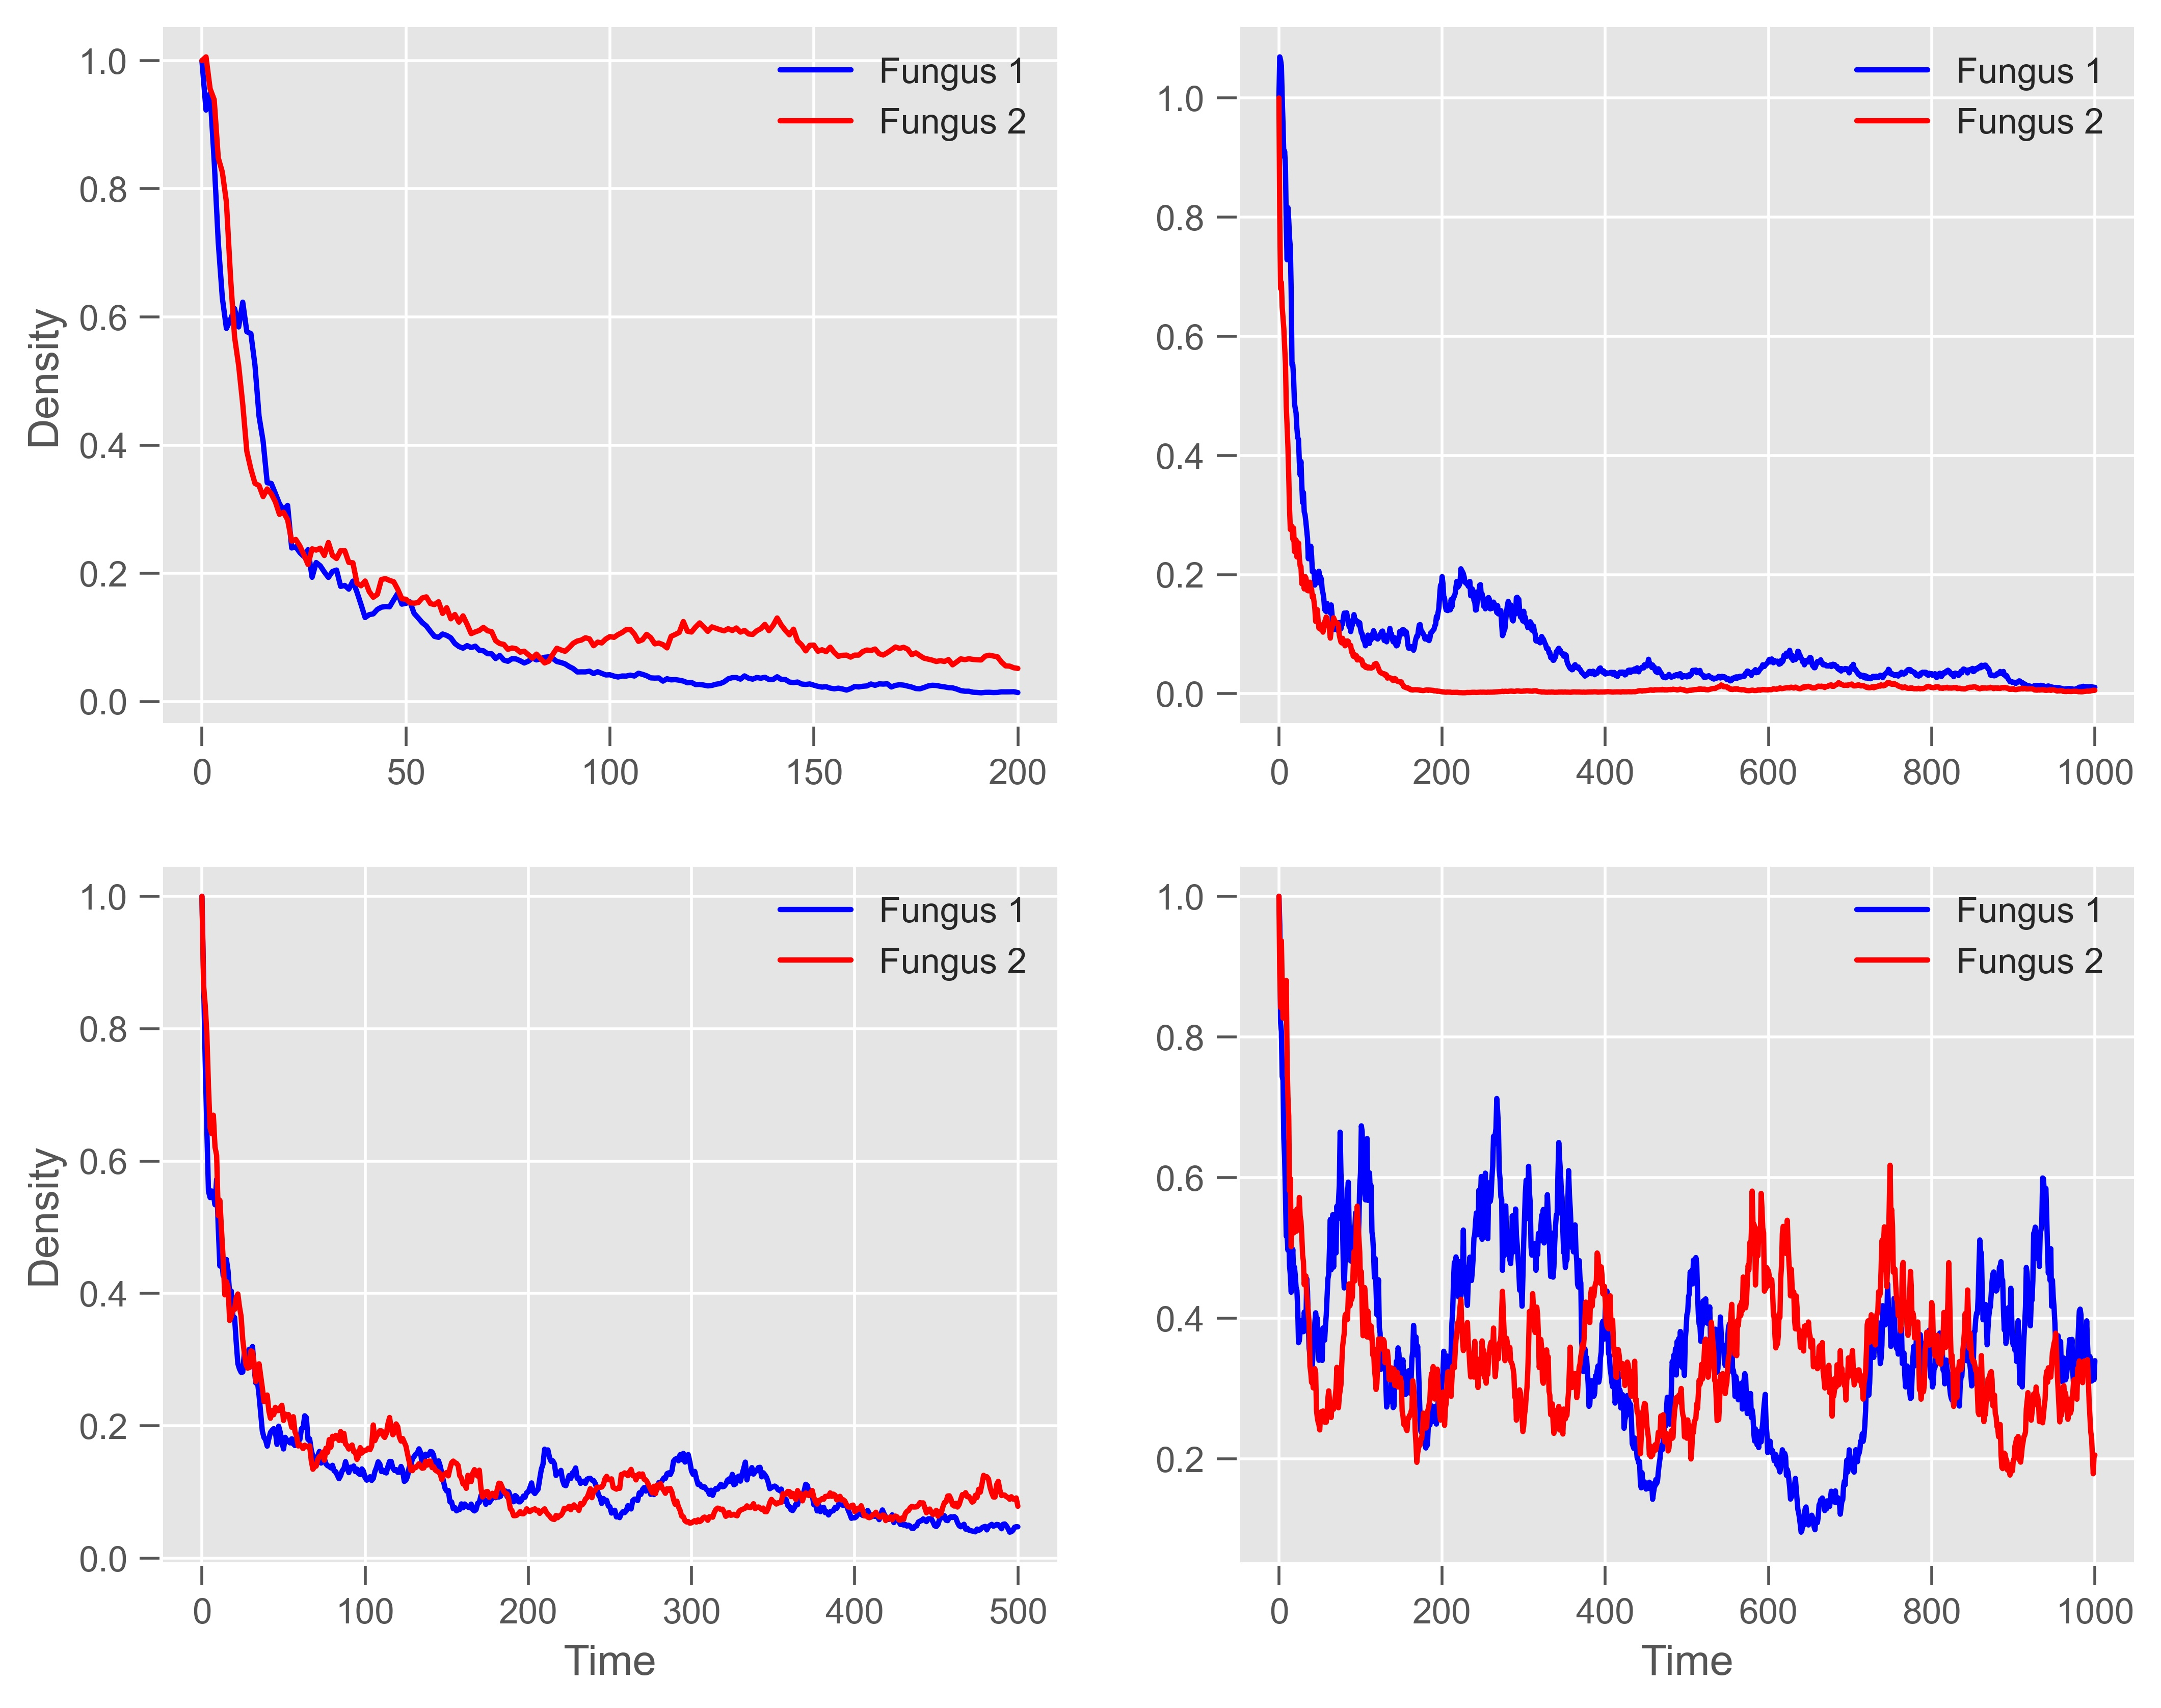
\includegraphics[width=0.6\textwidth]{./code/fig8.jpg}
    \caption{Dynamic change of Fungus 1 and 2}\label{fig8}
\end{figure}

For the first picture in Figure (\ref{fig8}):

$C_{0}(t)=0.2+0.01\sin t$

\begin{multicols}{5}
    $r_{10}=0.1$
    
    $r_{11}=0.5$
    
    $a_{11}=0.5$
    
    $a_{12}=0.5$
    
    $\sigma_{1}=0.2$

    $\sigma_{2}=0.2$
    
    $r_{20}=0.05$
    
    $r_{21}=0.6$
    
    $a_{21}=0.4$
    
    $a_{22}=0.5$

\end{multicols}

the second picture:

$C_{0}(t)=0.1+0.01\sin t$

\begin{multicols}{5}
    $r_{10}=0.1$
    
    $r_{11}=0.5$
    
    $a_{11}=0.5$
    
    $a_{12}=0.5$
    
    $\sigma_{1}=0.2$

    $\sigma_{2}=0.2$
    
    $r_{20}=0.05$
    
    $r_{21}=0.6$
    
    $a_{21}=0.4$
    
    $a_{22}=0.5$

\end{multicols}

the third picture:

$C_{0}(t)=0.001+0.001\sin t$

\begin{multicols}{5}
    $r_{10}=0.1$
    
    $r_{11}=0.5$
    
    $a_{11}=0.5$
    
    $a_{12}=0.5$
    
    $\sigma_{1}=0.2$

    $\sigma_{2}=0.2$
    
    $r_{20}=0.05$
    
    $r_{21}=0.6$
    
    $a_{21}=0.4$
    
    $a_{22}=0.5$

\end{multicols}

the fourth picture:

$C_{0}(t)=0.005+0.001\sin t$

\begin{multicols}{5}
    $r_{10}=0.4$
    
    $r_{11}=0.2$
    
    $a_{11}=0.5$
    
    $a_{12}=0.5$
    
    $\sigma_{1}=0.2$

    $\sigma_{2}=0.2$
    
    $r_{20}=0.3$
    
    $r_{21}=0.1$
    
    $a_{21}=0.4$
    
    $a_{22}=0.5$

\end{multicols}